% Comparator + hysteresis transfer sketch
\begin{circuitikz}[american, scale=0.85, transform shape]
\draw (0,0) node[op amp] (a) {};
\draw (a.-) to[short, -o] ++(-0.8,0) node[left] {$v_{\mathrm{in}}$};
\draw (a.+) -- ++(0,-0.9) coordinate (tap);
\draw (tap) to[R, l_=$R_1$] ++(-1.7,0) node[ground] {};
\draw (a.out) -- ++(0.9,0) coordinate (o) node[right] {$v_{\mathrm{out}}$};
\draw (o) -- ++(0,-0.9) to[R, l_=$R_2$] (tap);
\end{circuitikz}
\hspace{1.2cm}
\begin{tikzpicture}
\begin{axis}[width=0.55\linewidth, height=5cm,
  xlabel={$v_{\mathrm{in}}$ (V)}, ylabel={$v_{\mathrm{out}}$ (V)},
  xmin=-8, xmax=8, ymin=-13, ymax=13,
  xtick={-5,0,5}, xticklabels={$-V_T$,0,$+V_T$},
  ytick={-10.5,0,10.5}, yticklabels={$-V_{\mathrm{sat}}$,0,$+V_{\mathrm{sat}}$},
  grid=both, grid style={gray!25}]
% hysteresis loop
\addplot[blue, very thick, ->] coordinates {(-7,-10.5) (5,-10.5)};
\addplot[blue, very thick, ->] coordinates {(5,-10.5) (5,10.5)};
\addplot[blue, very thick, ->] coordinates {(7,10.5) (-5,10.5)};
\addplot[blue, very thick, ->] coordinates {(-5,10.5) (-5,-10.5)};
\node[font=\footnotesize, text=gray] at (axis cs:0,12) {$V_T = \tfrac{R_1}{R_1+R_2}V_{\mathrm{sat}}$};
\end{axis}
\end{tikzpicture}
